% !TEX TS-program = xelatex
% !TEX encoding = UTF-8
% !Mode:: "TeX:UTF-8"

\documentclass[onecolumn, oneside, ctexart]{SUSTechHomework}
\setlength{\parindent}{2em}
\linespread{1.5}
\usepackage{karnaugh-map}
\usepackage{float}
\usepackage{circuitikz}
\ctikzset{logic ports=ieee}
\usetikzlibrary{calc}

\coursecode{CS207}
\coursename{Digital Logic}
\title{Assignment 2}
\date{Nov. 1, 2021}

\lstset{language=verilog}

\begin{document}
  \maketitle
  \section{DIGITAL DESIGN THEORY}
\subsection*{Q. 1}
\paragraph{(a)}
Let $F_1=\Sigma m_{i}$ and $F_2=\Sigma m_{j}$, then $E=F_1+F_2=\Sigma m_{i}+\Sigma m_{j}=\Sigma (m_{i}+m_{j})$, which is the sum of the minterms of $F_1$ and $F_2$.
\vspace{-1em}
\paragraph{(b)}
Let $F_1=\Sigma m_{i}$ and $F_2=\Sigma m_{j}$, then $G=F_1\cdot F_2=\Sigma m_{i}\cdot \Sigma m_{j}=\Sigma_i\Sigma_j(m_i\cdot m_j)$, where $m_i\cdot m_j=\left\{
\begin{aligned}
0(i\not=j)\\
1(i=j)
\end{aligned}
\right.$, in this case only the minterms where both in (say, common to) $F_1$ and $F_2$, a.k.a. appear to have the same $i$ and $j$ can be $i$ in $G$.

\subsection*{Q. 2}
\paragraph{(a)}
$F(x,y,z)=\Pi(0,1,2,4,6)$
\vspace{-1em}
\paragraph{(b)}
$F(A,B,C,D)=\Sigma(0,1,2,4,6,7,9,10,13,14)$

\subsection*{Q. 3}
\subsubsection*{(a)}
\paragraph{Converting to min/max-terms}
\begin{align*}
(b'+d)(a'+b'+c)(a'+c)
&=b'a'a'+b'a'c+b'b'a'+b'b'c+b'ca'+b'cc+\\
&\qquad da'a'+da'c+db'a'+db'c+dca'+dcc\\
&=a'b'+a'b'c+a'b'+b'c+a'b'c+b'c+a'd+a'cd+a'b'd+b'cd+a'cd+cd\\
&=a'b'+a'b'c+b'c+a'd+a'cd+a'b'd+b'cd+cd\\
&=a'b'+b'c+a'd+a'b'd+cd\\
&=a'b'+b'c+a'd+cd
\end{align*}
\pagebreak
\paragraph{Using K-map}
\vspace{-1em}
\begin{center}
\begin{karnaugh-map}[4][4][1][$cd$][$ab$]
\maxterms{4,12,8,13,9,6,14}
\implicant{0}{2}
\implicant{3}{11}
\implicant{1}{7}
\implicantedge{3}{2}{11}{10}
\end{karnaugh-map}
\end{center}
\vspace{-2em}
\begin{align*}
(b'+d)(a'+b'+c)(a'+c)&=a'b'+cd+a'd+b'c
\end{align*}

\subsubsection*{(b)}
\vspace{-5em}
\begin{align*}
xy+x'z'+x'yz
&=xy(z+z')+x'(y+y')z'+x'yz\\
&=xyz+xyz'+x'yz'+x'y'z'+x'yz\\
&=\Sigma(0,2,3,6,7)\\
&=\Pi(1,4,5)\\
&=(x+y+z')(x'+y+z)(x'+y+z')
\end{align*}

\subsection*{Q. 4}
\subsubsection*{(a)}
\vspace{-5em}
\begin{align*}
y'z'+yz'+x'z
&=(y'+y)z'+x'z &\text{(LHS)}\\
&=z'+x'z\\
&=x'+z'\\
x'+xz'&=x'+z'&\text{(RHS)}
\end{align*}
\centerline{Thus LHS = RHS, the equation is true.}

\subsubsection*{(b)}
\vspace{-5em}
\begin{align*}
x'y+xz+y'z'
&=x'y(z+z')+x(y+y')z+(x+x')y'z' &\text{(LHS)}\\
&=x'yz+x'yz'+xyz+xy'z+xy'z'+x'y'z'\\
&=(xy'z+xy'z')+(x'yz'+x'y'z')+(x'yz+xyz)\\
&=xy'+x'z'+yz &\text{(RHS)}
\end{align*}
\centerline{Thus LHS = RHS, the equation is true.}


\subsection*{Q. 5}
\subsubsection*{(a)}
\begin{center}
\begin{karnaugh-map}[4][4][1][$yz$][$wx$]
\minterms{8,10,12,13,14}
\implicantedge{12}{8}{14}{10}
\implicant{12}{13}
\end{karnaugh-map}
\end{center}
\vspace{-4em}
\begin{align*}
F (w, x, y, z)=(wy'z'+wyz')+wxy'=wz'+wxy'
\end{align*}

\subsubsection*{(b)}
\begin{center}
\begin{karnaugh-map}[4][4][1][$CD$][$AB$]
\minterms{0,2,5,7,8,10,13,15}
\implicant{5}{15}
\implicantcorner
\end{karnaugh-map}
\end{center}
\vspace{-4em}
\begin{align*}
F (A, B, C, D)=BD+B'D'
\end{align*}

\subsubsection*{(c)}
\begin{center}
\begin{karnaugh-map}[4][4][1][$CD$][$AB$]
\minterms{11,13,15,9,7,8,12}
\implicant{12}{9}
\implicant{13}{11}
\implicant{7}{15}
\end{karnaugh-map}
\end{center}
\vspace{-4em}
\begin{align*}
AB'CD + AD + AC' + BCD=AC'+AD+BCD
\end{align*}

\subsubsection*{(d)}
\begin{center}
\begin{karnaugh-map}[4][4][1][$CD$][$AB$]
\minterms{1,15,4,5,10,11,9}
\implicant{4}{5}
\implicantedge{1}{1}{9}{9}
\implicant{11}{10}
\implicant{15}{11}
\end{karnaugh-map}
\end{center}
\vspace{-4em}
\begin{align*}
A'B'C'D + ABCD + A'BC' + AB'C + AB'D
=A'BC'+B'C'D+ACD+AB'C
\end{align*}

\subsection*{Q. 6}
\subsubsection*{(a)}
\begin{center}
\begin{karnaugh-map}[4][4][1][$CD$][$AB$]
\maxterms{0,4,12,8,5}
\maxterms{3,7,15,11}
\implicant{0}{8}
\implicant{3}{11}
\implicant{4}{5}
\end{karnaugh-map}
\end{center}
\vspace{-4em}
\begin{align*}
F(A, B, C, D)=(C+D)(C'+D')(A+B'+C)
\end{align*}
\centerline{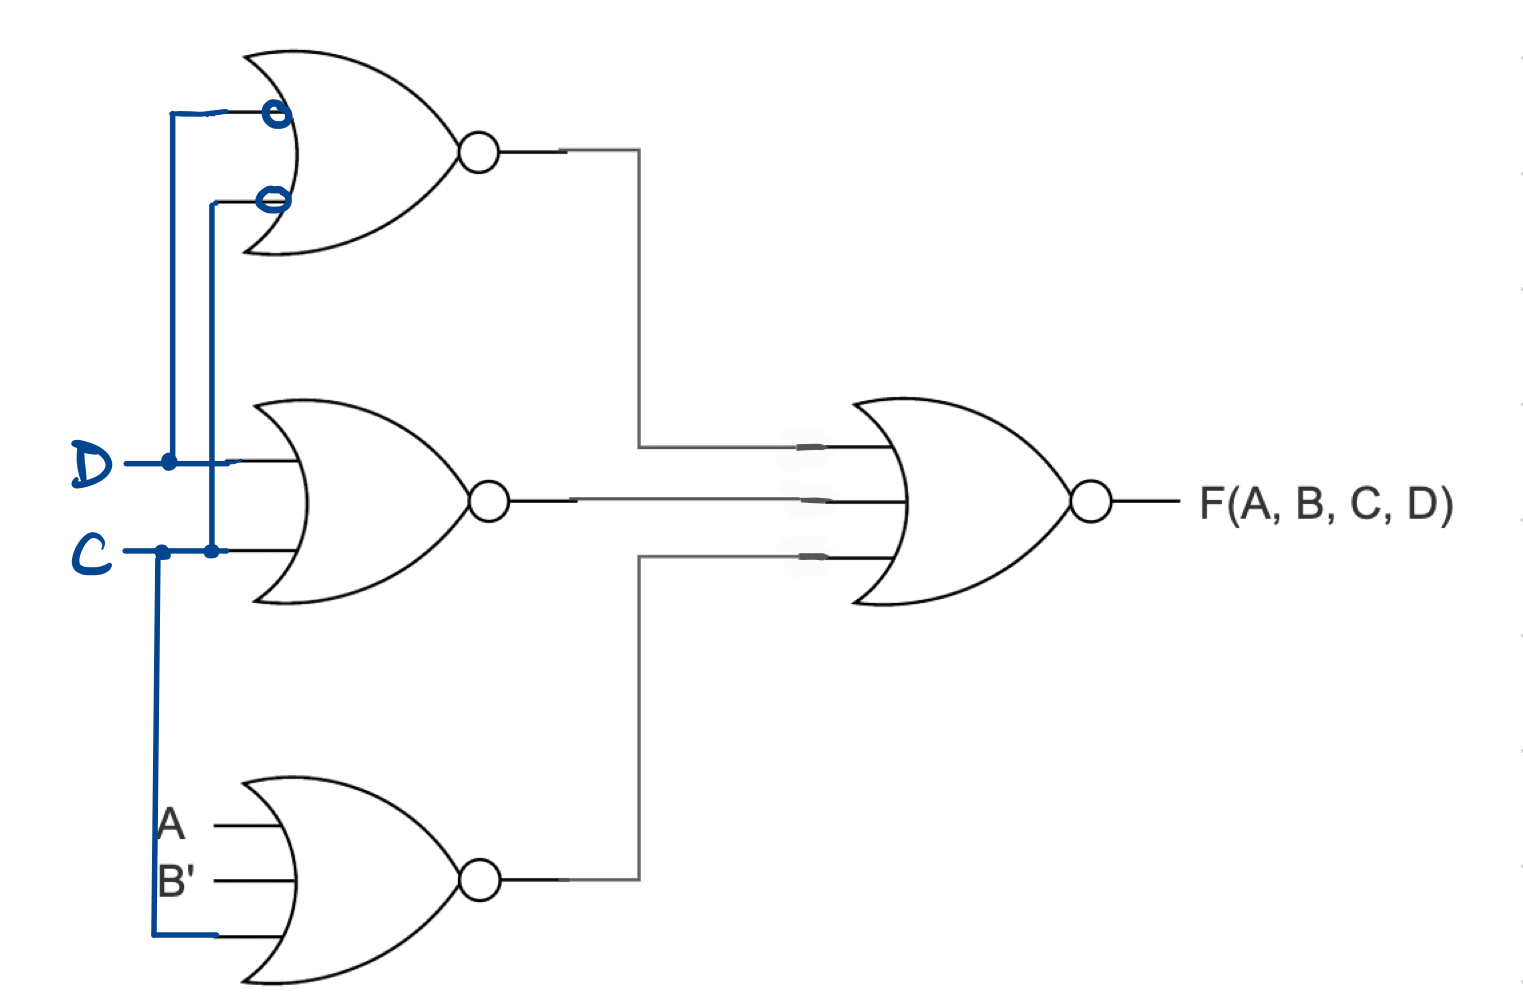
\includegraphics[width=0.4\textwidth]{6a.jpeg}\quad or\quad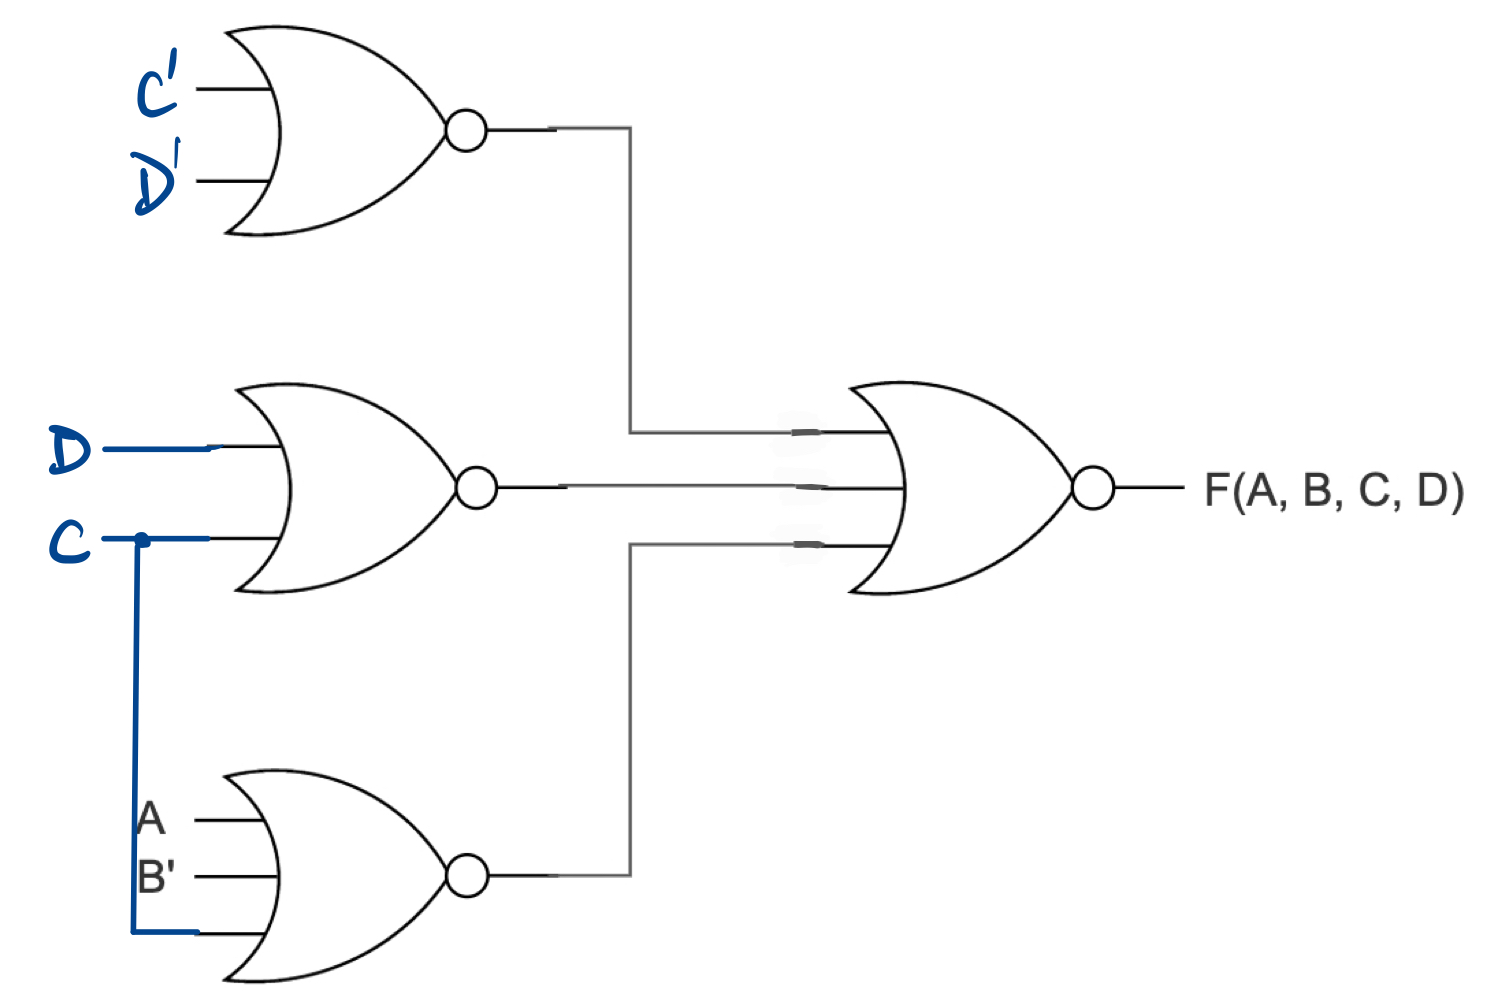
\includegraphics[width=0.4\textwidth]{6a1.jpeg}}
	
\subsubsection*{(b)}
\begin{center}
\begin{karnaugh-map}[4][4][1][$CD$][$AB$]
\maxterms{8,9}
\implicant{8}{9}
\end{karnaugh-map}
\end{center}
\vspace{-4em}
\begin{align*}
F(A, B, C, D)=A'+B+C
\end{align*}
\centerline{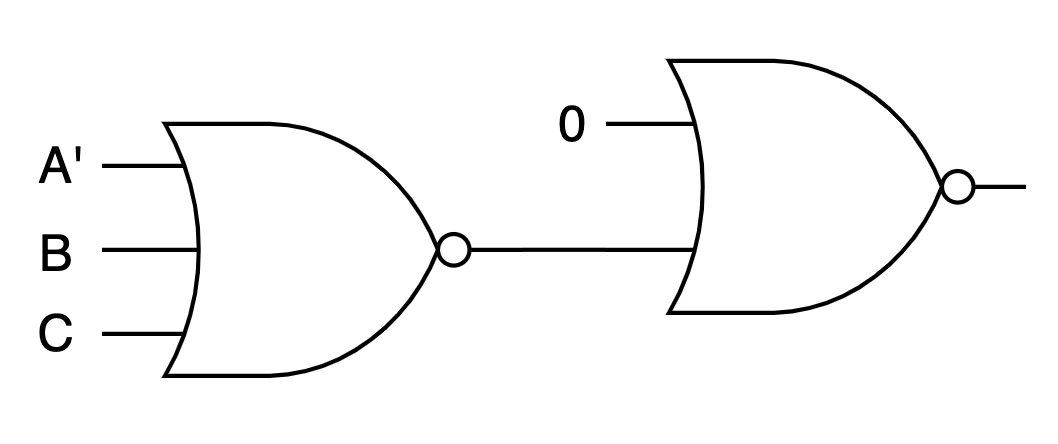
\includegraphics[width=0.4\textwidth]{6b}}

\subsection*{Q. 7}
\subsubsection*{(a)}
\begin{center}
\begin{karnaugh-map}[4][4][1][$CD$][$AB$]
\manualterms{d,0,1,0,1,0,d,1,d,0,1,0,1,0,0,0}
\implicant{0}{8}
\implicantcorner
\implicant{7}{6}
\end{karnaugh-map}
\end{center}
\vspace{-4em}
\begin{align*}
F(A, B, C, D)
&=C'D'+B'D'+A'BC\\
&=\Sigma(0,2,4,6,7,8,10,12)
\end{align*}

\subsubsection*{(b)}
\begin{center}
\begin{karnaugh-map}[4][4][1][$CD$][$AB$]
\manualterms{d,d,1,0,1,d,0,0,d,0,1,0,1,0,1,0}
\implicant{0}{8}
\implicantcorner
\implicantedge{12}{8}{14}{10}
\end{karnaugh-map}
\end{center}
\vspace{-4em}
\begin{align*}
F(A, B, C, D)
&=B'D'+C'D'+AD'\\
&=\Sigma(0,2,4,8,10,12,14)
\end{align*}

\subsection*{Q. 8}
\vspace{-5em}
\begin{align*}
F&=A'BC'D+AB'CD'+ABC'D'+A'B'CD\\
&=(A'D+AD')BC'+(AD'+A'D)B'C\\
&=(A'D+AD')(BC'+B'C)\\
&=(A\oplus D)(B\oplus C)
\end{align*}
\centerline{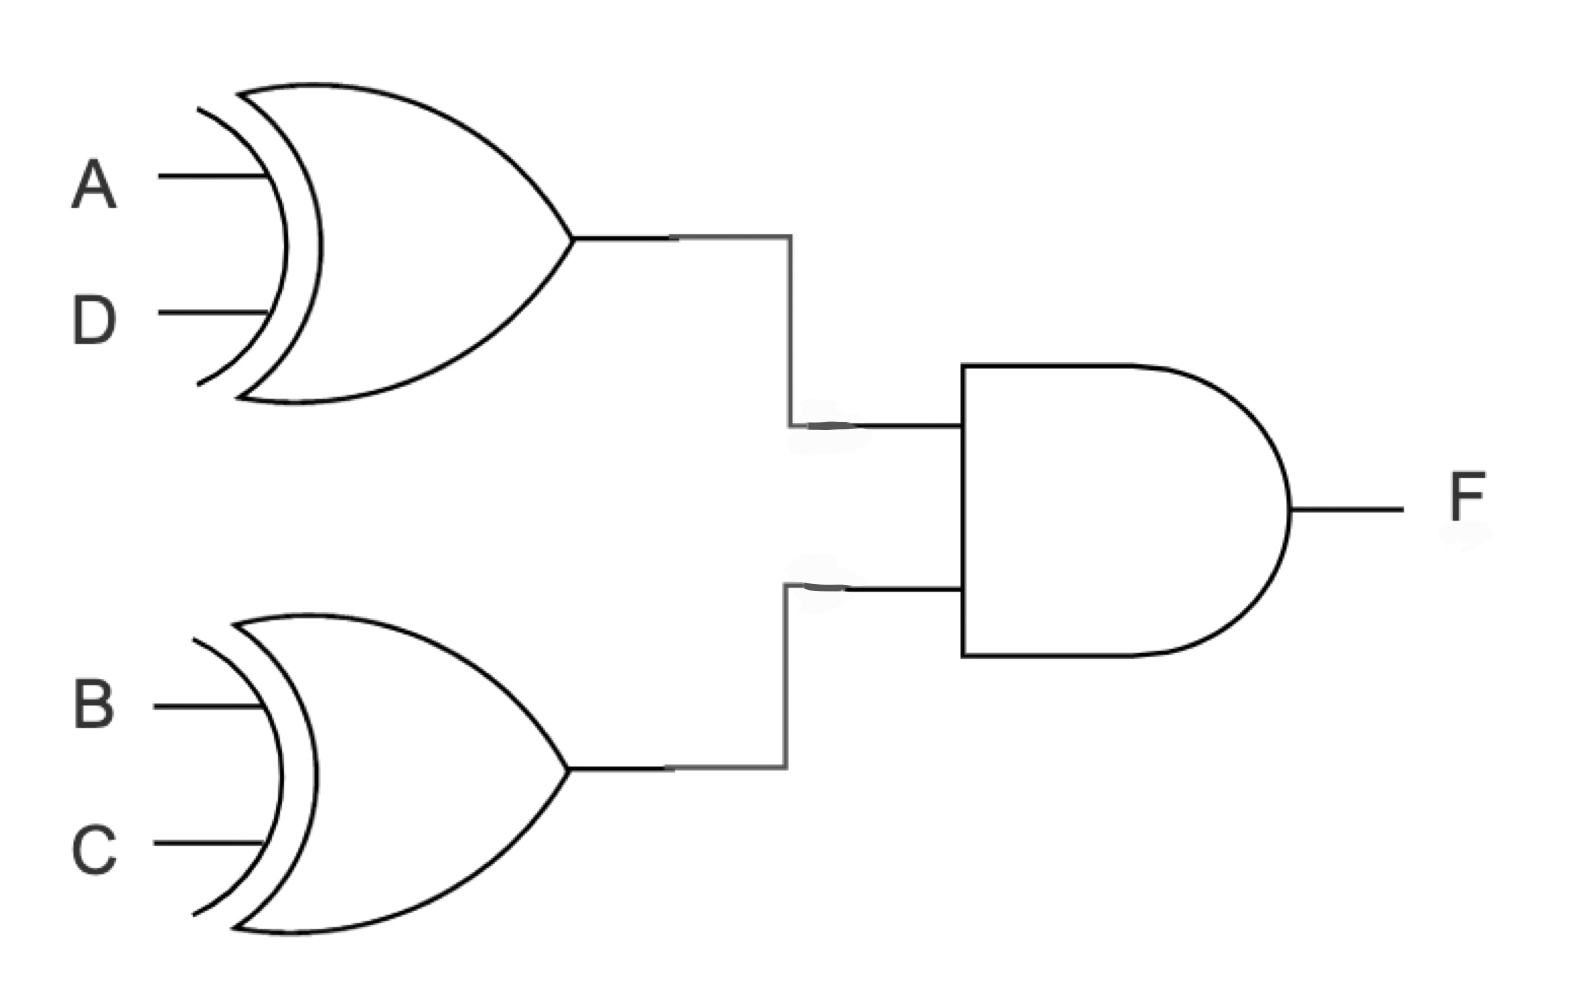
\includegraphics[width=0.4\textwidth]{8.jpeg}}
\pagebreak

\section{DIGITAL DESIGN LAB}
\subsection{Task 1}
\begin{lstlisting}
`timescale 1ns / 1ps

module seg_tube (
    input [3:0] id,
    output reg [7:0] seg_out
);
    always @* begin
        case(id)
            0: seg_out=8'b1100_0000;          // 0
            1: seg_out=8'b1111_1001;          // 1
            2: seg_out=8'b1010_0100;          // 2
            3: seg_out=8'b1011_0000;          // 3
            default: seg_out = 8'b1111_1111;  // off
        endcase
    end
endmodule

module enc (
    input [3:0] bell,
    input hi_fst,
    output [7:0] seg_out, seg_en
);
    assign seg_en = 8'b1111_1110;
    reg [3:0] dispid;
    always @* begin
        case(hi_fst)
            1: begin
                casex(bell)
                    'b0000: dispid <= 'b100;  // invalid flag
                    'b0001: dispid <= 0;
                    'b001x: dispid <= 1;
                    'b01xx: dispid <= 2;
                    'b1xxx: dispid <= 3;
                endcase
            end
            0: begin
                casex(bell)
                    'b0000: dispid <= 'b100;
                    'b1000: dispid <= 3;
                    'bx100: dispid <= 2;
                    'bxx10: dispid <= 1;
                    'bxxx1: dispid <= 0;
                endcase
            end
        endcase
    end
    seg_tube st(.id(dispid), .seg_out(seg_out));
endmodule

\end{lstlisting}
\vspace{-3em}
\par The design file contains two module, the assistant module that helps converting an input id into the seg-tube-code, while the main module \emph{mux} takes a priority switch and the input switches, then select the one having the highest priority and convert it into seg-tube-code. To make it elegant (that can use the assistant module \textit{seg\_tube}), though the code of wards 0 - 3 can be represented in a 2-bit binary number, I use a 3-bit register that can represent the no-switch-state. (say, \emph{dispid} actually acts as \\\centerline{\{disable\_output, id[1], id[0]\}}\\, this is only for convenience.)\\

\begin{lstlisting}
# seg_tube
set_property IOSTANDARD LVCMOS33 [get_ports {seg_en[0]}]
set_property IOSTANDARD LVCMOS33 [get_ports {seg_en[1]}]
set_property IOSTANDARD LVCMOS33 [get_ports {seg_en[2]}]
set_property IOSTANDARD LVCMOS33 [get_ports {seg_en[3]}]
set_property IOSTANDARD LVCMOS33 [get_ports {seg_en[4]}]
set_property IOSTANDARD LVCMOS33 [get_ports {seg_en[5]}]
set_property IOSTANDARD LVCMOS33 [get_ports {seg_en[6]}]
set_property IOSTANDARD LVCMOS33 [get_ports {seg_en[7]}]
set_property IOSTANDARD LVCMOS33 [get_ports {seg_out[0]}]
set_property IOSTANDARD LVCMOS33 [get_ports {seg_out[1]}]
set_property IOSTANDARD LVCMOS33 [get_ports {seg_out[2]}]
set_property IOSTANDARD LVCMOS33 [get_ports {seg_out[3]}]
set_property IOSTANDARD LVCMOS33 [get_ports {seg_out[4]}]
set_property IOSTANDARD LVCMOS33 [get_ports {seg_out[5]}]
set_property IOSTANDARD LVCMOS33 [get_ports {seg_out[6]}]
set_property IOSTANDARD LVCMOS33 [get_ports {seg_out[7]}]
set_property PACKAGE_PIN A18 [get_ports {seg_en[7]}]
set_property PACKAGE_PIN A20 [get_ports {seg_en[6]}]
set_property PACKAGE_PIN B20 [get_ports {seg_en[5]}]
set_property PACKAGE_PIN E18 [get_ports {seg_en[4]}]
set_property PACKAGE_PIN F18 [get_ports {seg_en[3]}]
set_property PACKAGE_PIN D19 [get_ports {seg_en[2]}]
set_property PACKAGE_PIN E19 [get_ports {seg_en[1]}]
set_property PACKAGE_PIN C19 [get_ports {seg_en[0]}]
set_property PACKAGE_PIN E13 [get_ports {seg_out[7]}]
set_property PACKAGE_PIN C15 [get_ports {seg_out[6]}]
set_property PACKAGE_PIN C14 [get_ports {seg_out[5]}]
set_property PACKAGE_PIN E17 [get_ports {seg_out[4]}]
set_property PACKAGE_PIN F16 [get_ports {seg_out[3]}]
set_property PACKAGE_PIN F14 [get_ports {seg_out[2]}]
set_property PACKAGE_PIN F13 [get_ports {seg_out[1]}]
set_property PACKAGE_PIN F15 [get_ports {seg_out[0]}]

# priority/bell switchs
set_property IOSTANDARD LVCMOS33 [get_ports {bell[0]}]
set_property IOSTANDARD LVCMOS33 [get_ports {bell[1]}]
set_property IOSTANDARD LVCMOS33 [get_ports {bell[2]}]
set_property IOSTANDARD LVCMOS33 [get_ports {bell[3]}]
set_property PACKAGE_PIN T5 [get_ports {bell[3]}]
set_property PACKAGE_PIN T4 [get_ports {bell[2]}]
set_property PACKAGE_PIN R4 [get_ports {bell[1]}]
set_property PACKAGE_PIN W4 [get_ports {bell[0]}]
set_property IOSTANDARD LVCMOS33 [get_ports hi_fst]
set_property PACKAGE_PIN U5 [get_ports hi_fst]
set_property DRIVE 12 [get_ports {seg_en[7]}]
set_property DRIVE 12 [get_ports {seg_en[6]}]
set_property DRIVE 12 [get_ports {seg_en[5]}]
set_property DRIVE 12 [get_ports {seg_en[4]}]
set_property DRIVE 12 [get_ports {seg_en[3]}]
set_property DRIVE 12 [get_ports {seg_en[2]}]
set_property DRIVE 12 [get_ports {seg_en[1]}]
set_property DRIVE 12 [get_ports {seg_en[0]}]
\end{lstlisting}
\vspace{-3em}
\par Here we set the right-most 4 switches as the wards' bell input, and the $5^{\text{th}}$ switch as the priority switch.
\begin{figure*}[!h]
	\centering
	\begin{subfigure}[b]{0.8\textwidth}
		\centerline{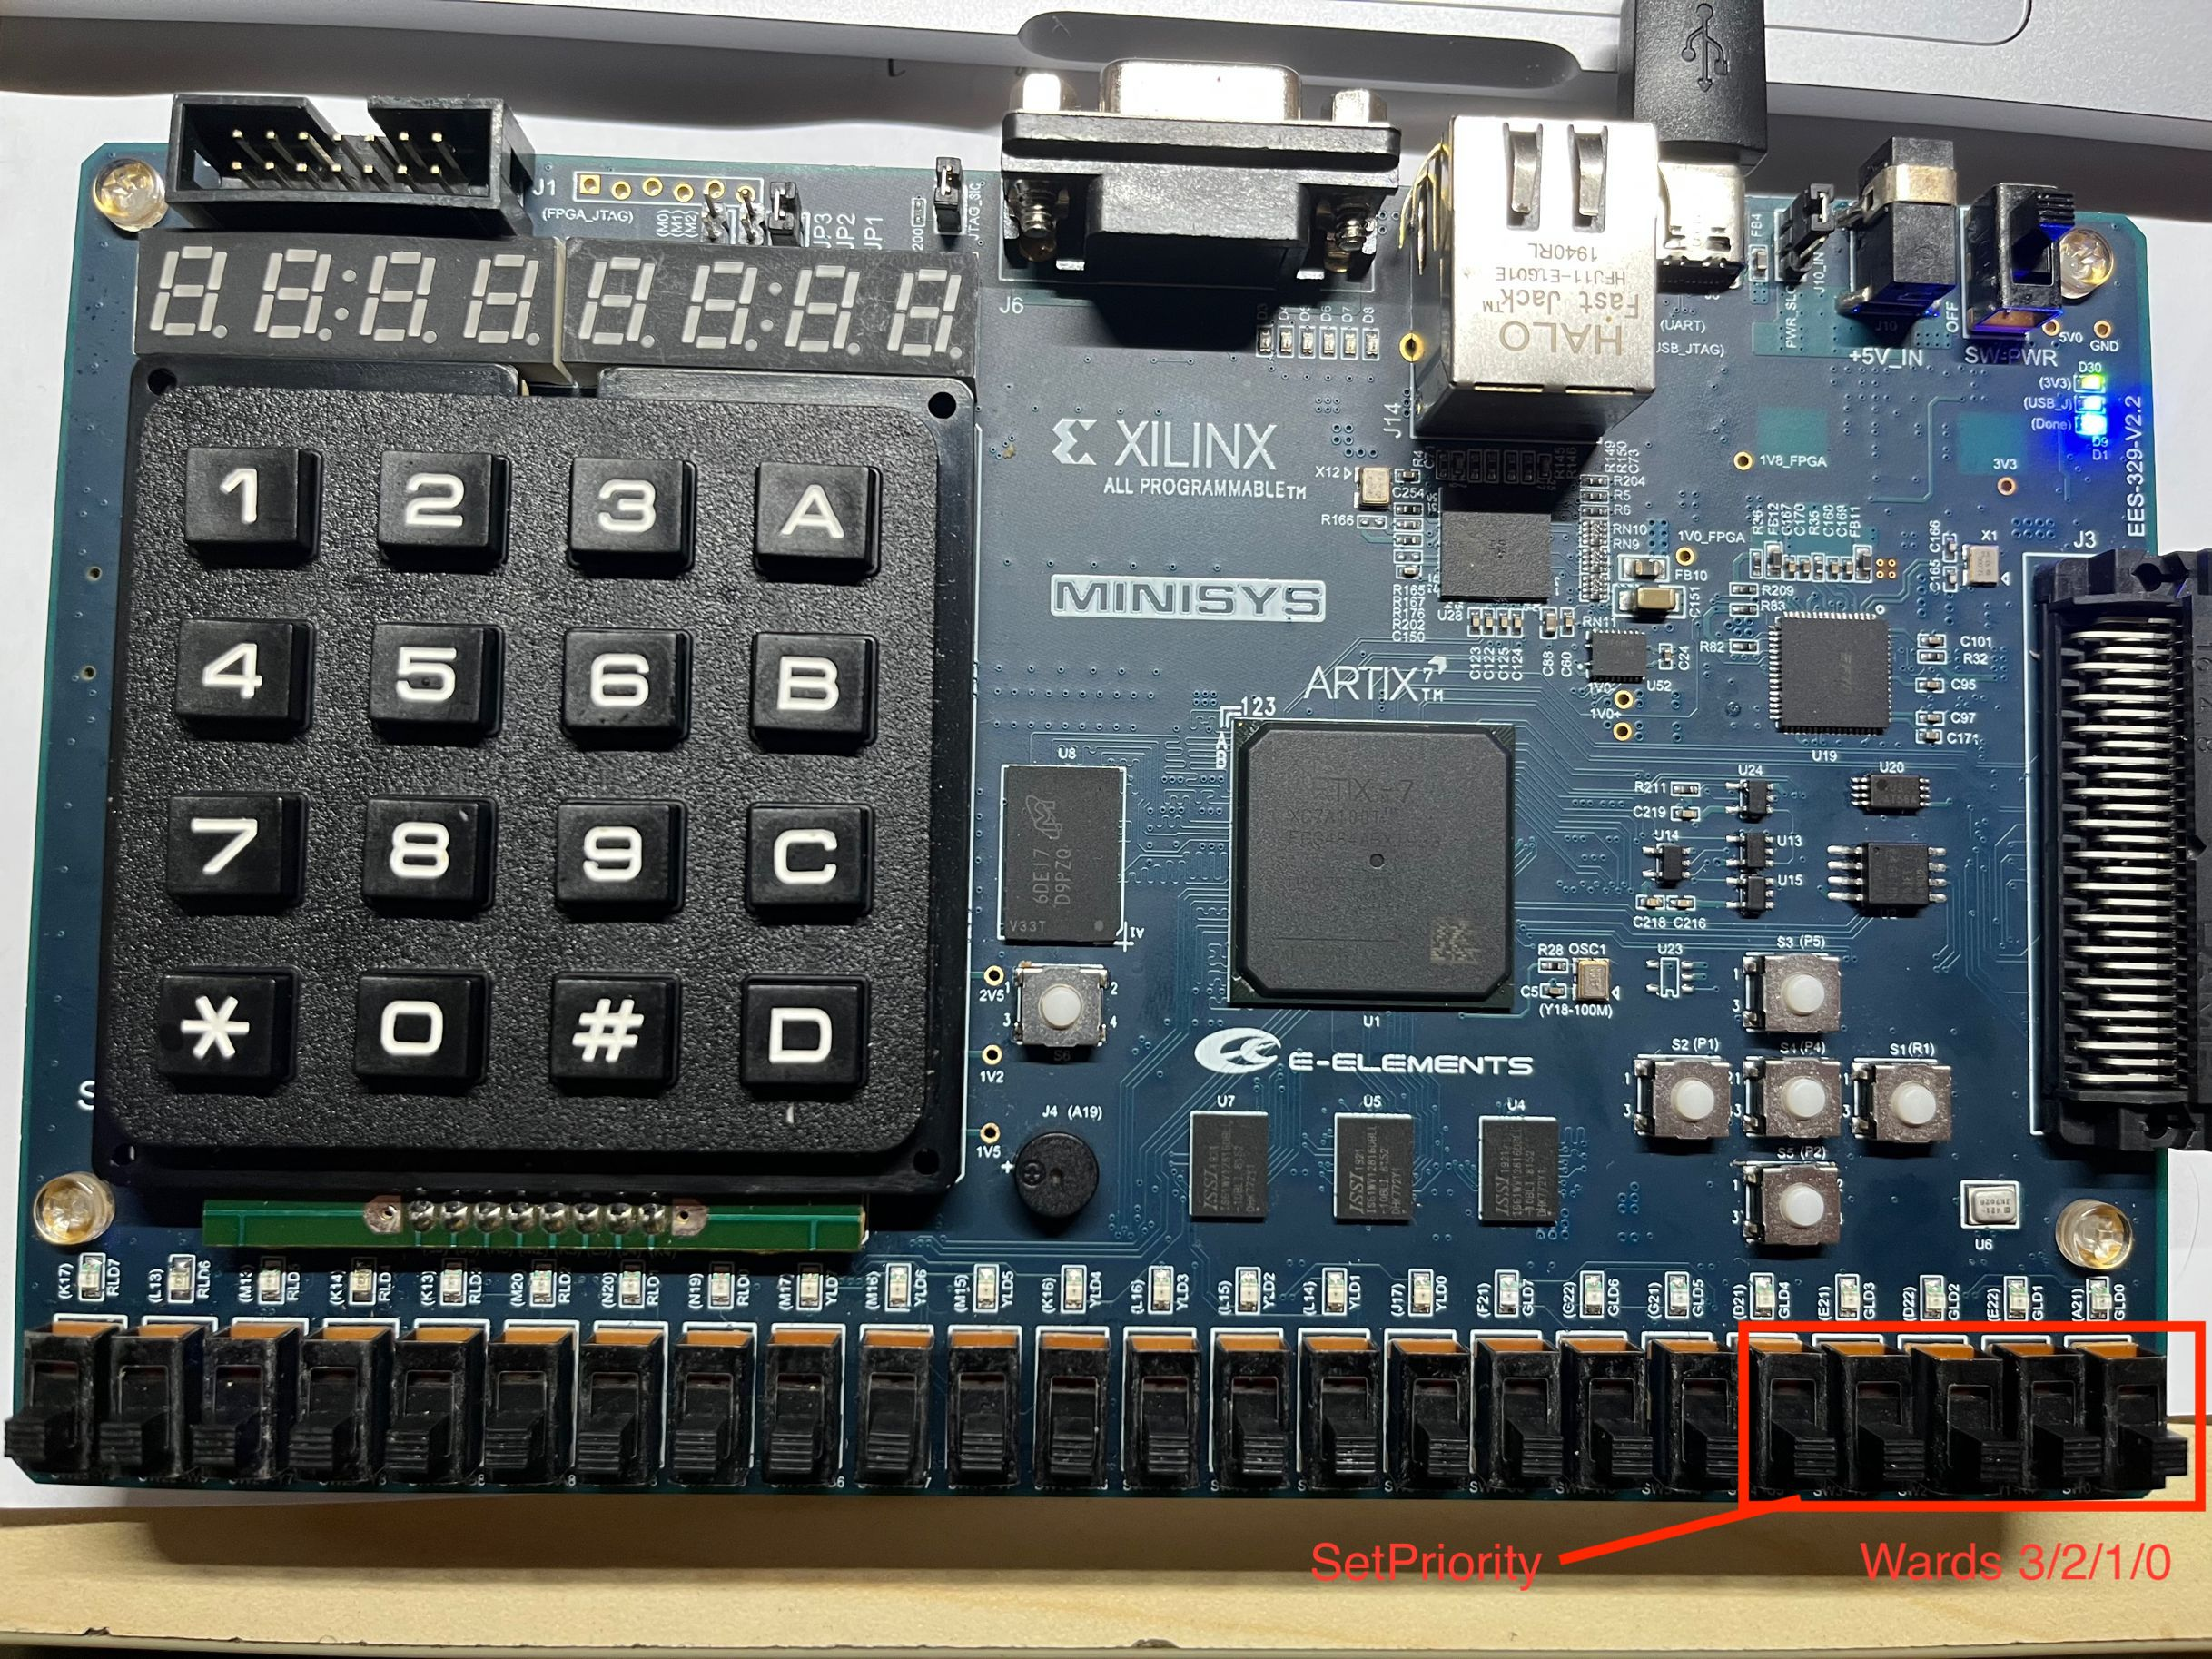
\includegraphics[width=0.6\textwidth]{./t1/noinp.jpg}}
		\caption{When no ward press the bell, display nothing}
	\end{subfigure}
	\begin{subfigure}[b]{\textwidth}
		\centerline{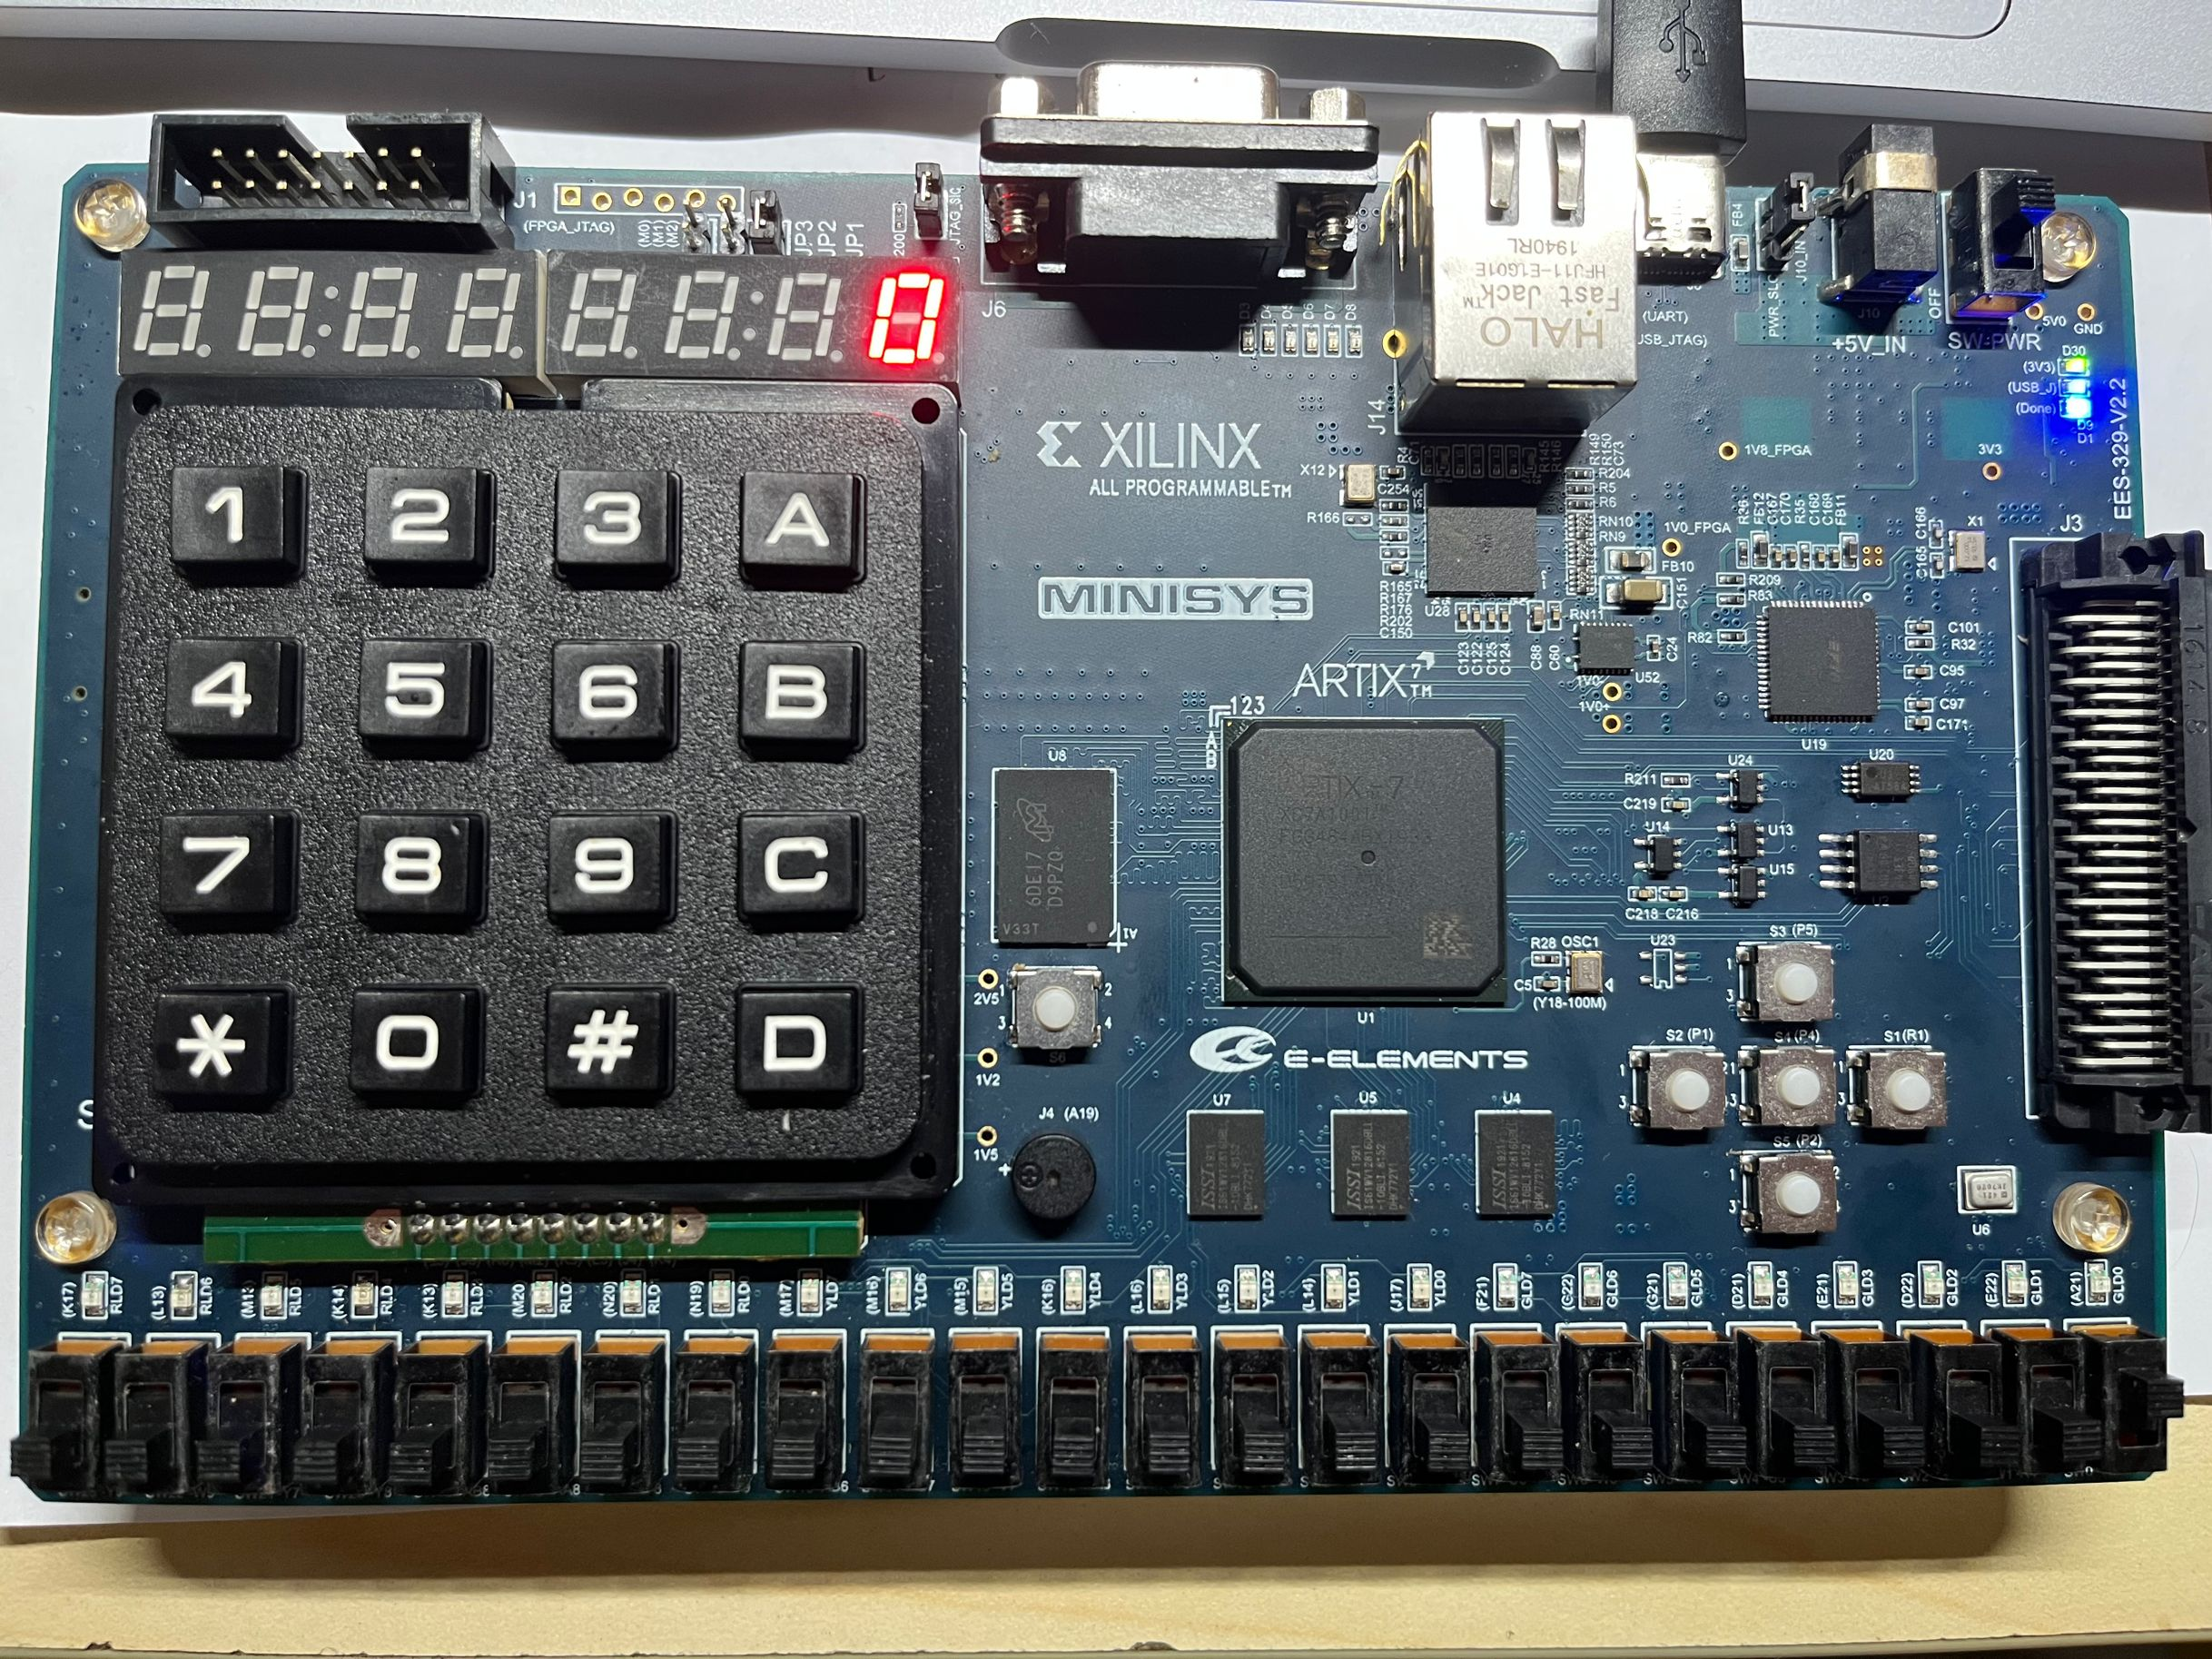
\includegraphics[width=0.35\textwidth]{./t1/lof1.jpg}\qquad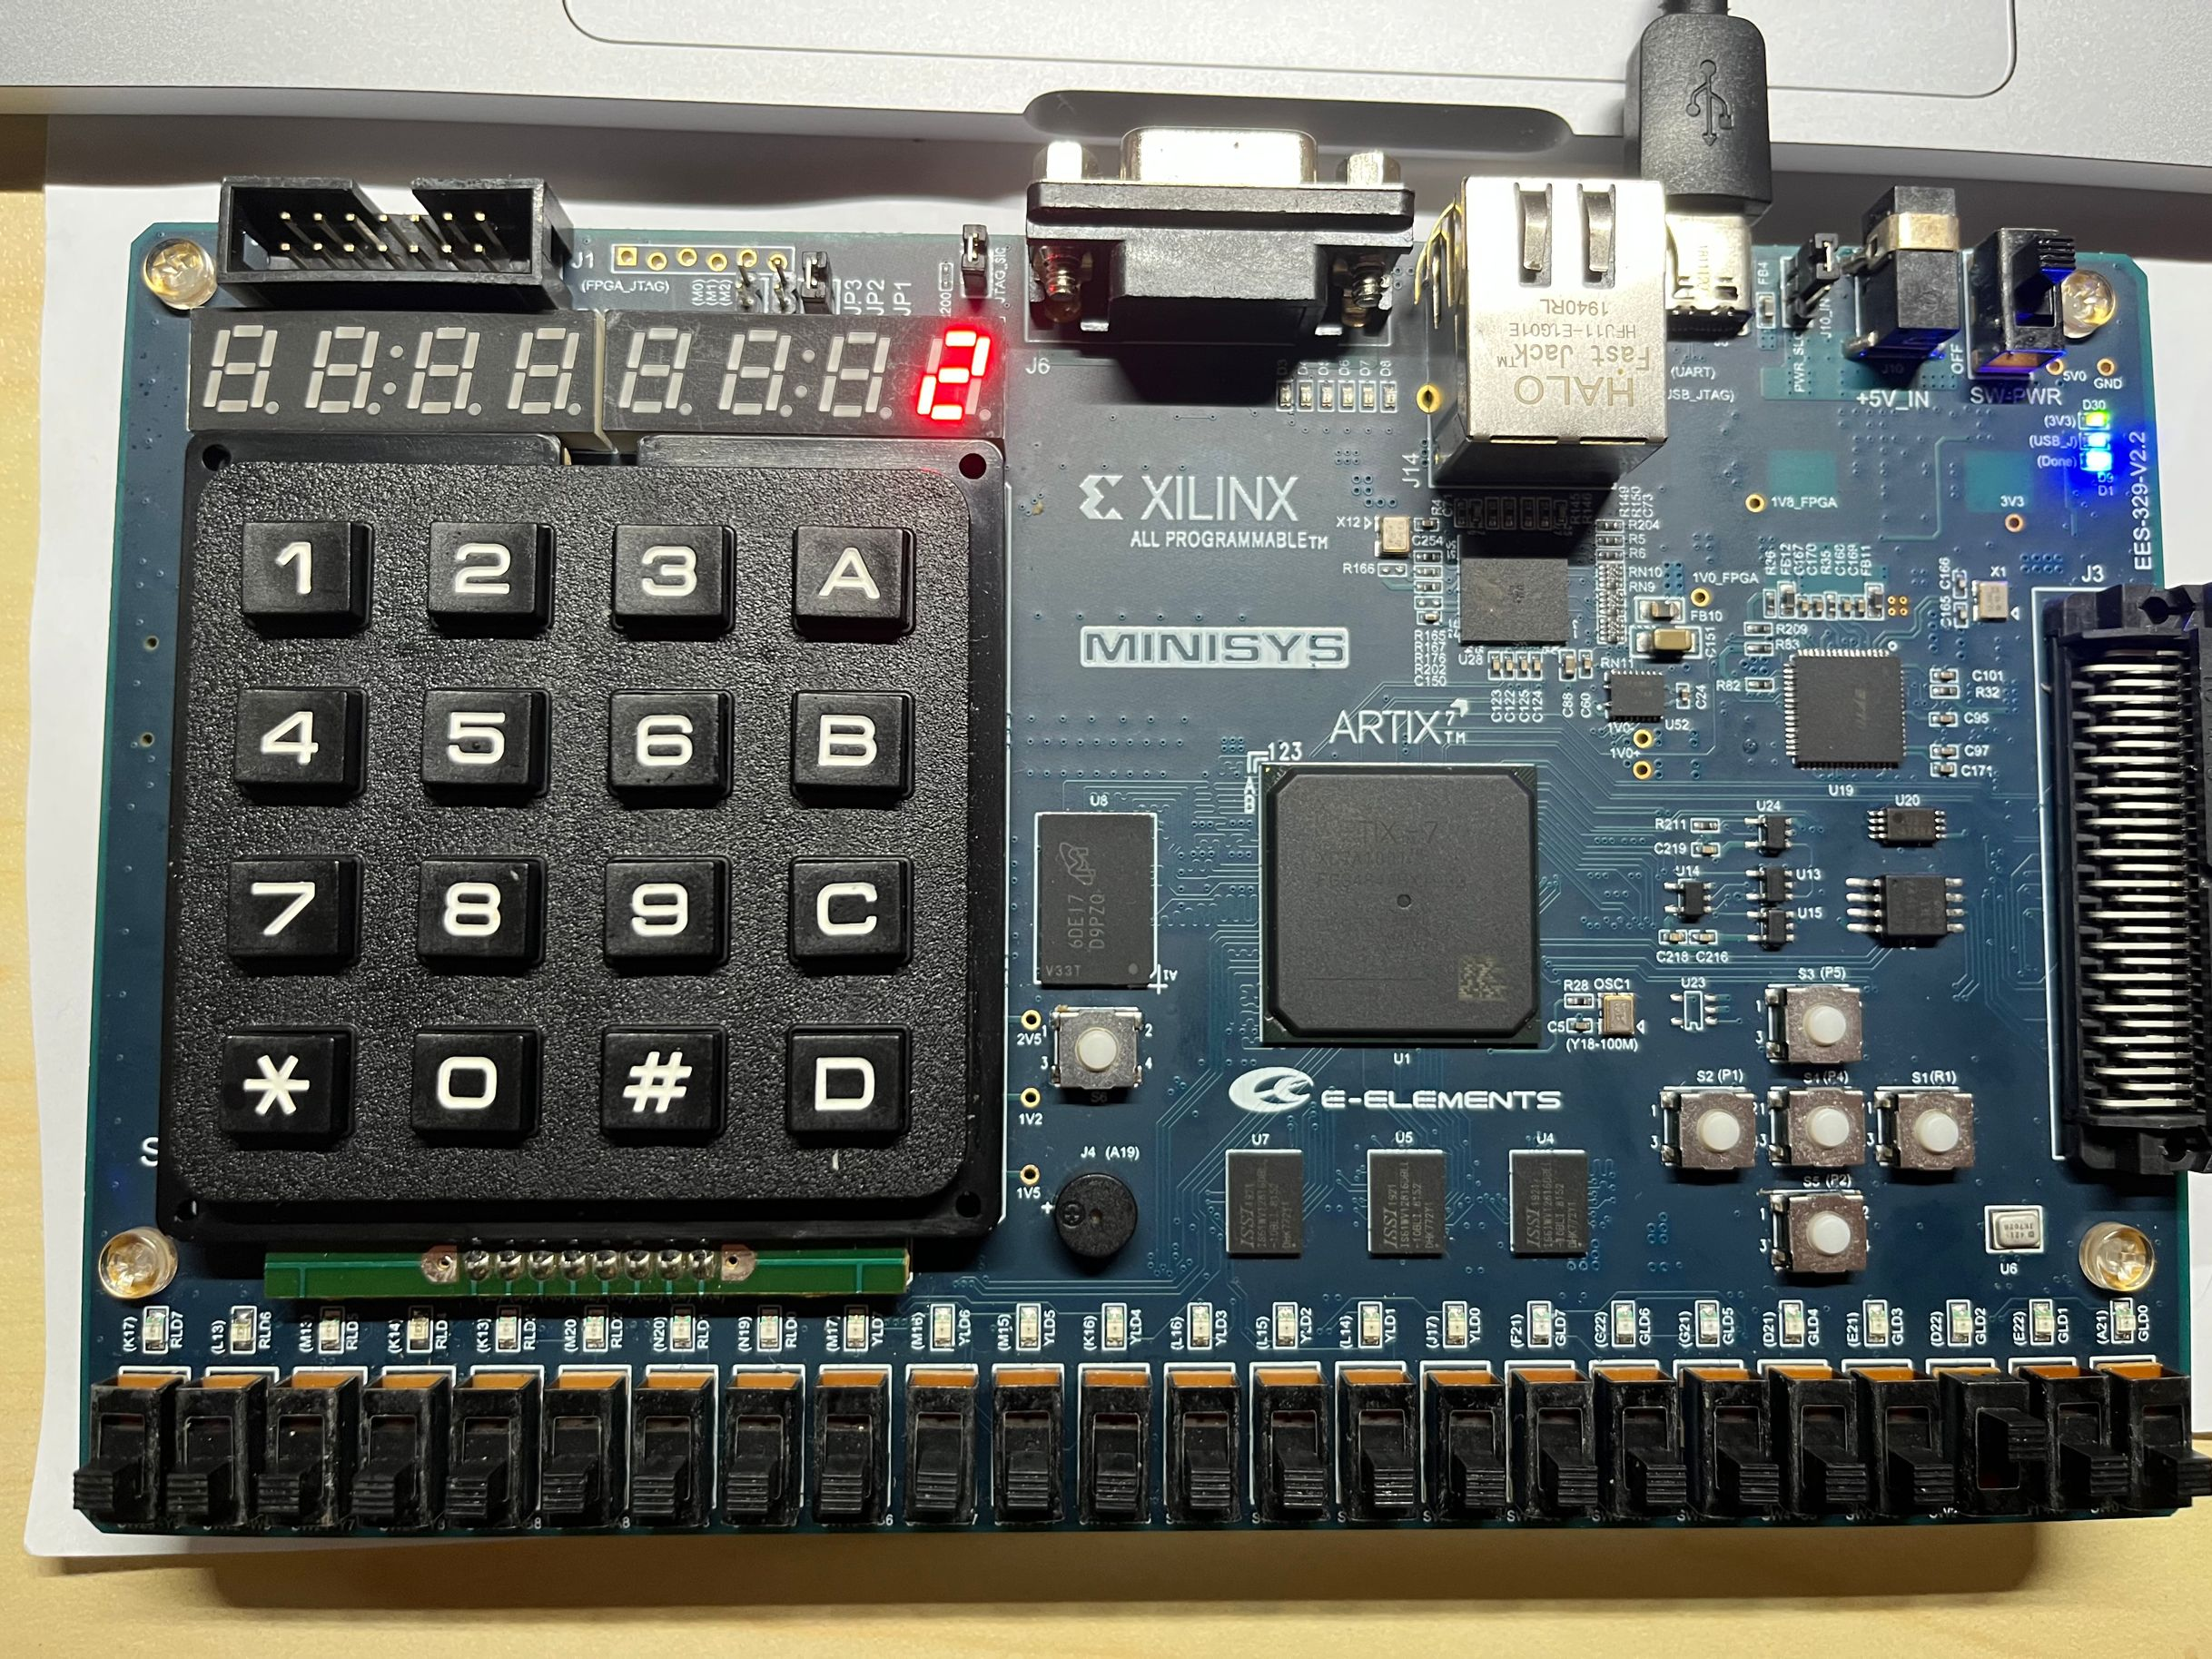
\includegraphics[width=0.35\textwidth]{./t1/lof2.jpg}
			\qquad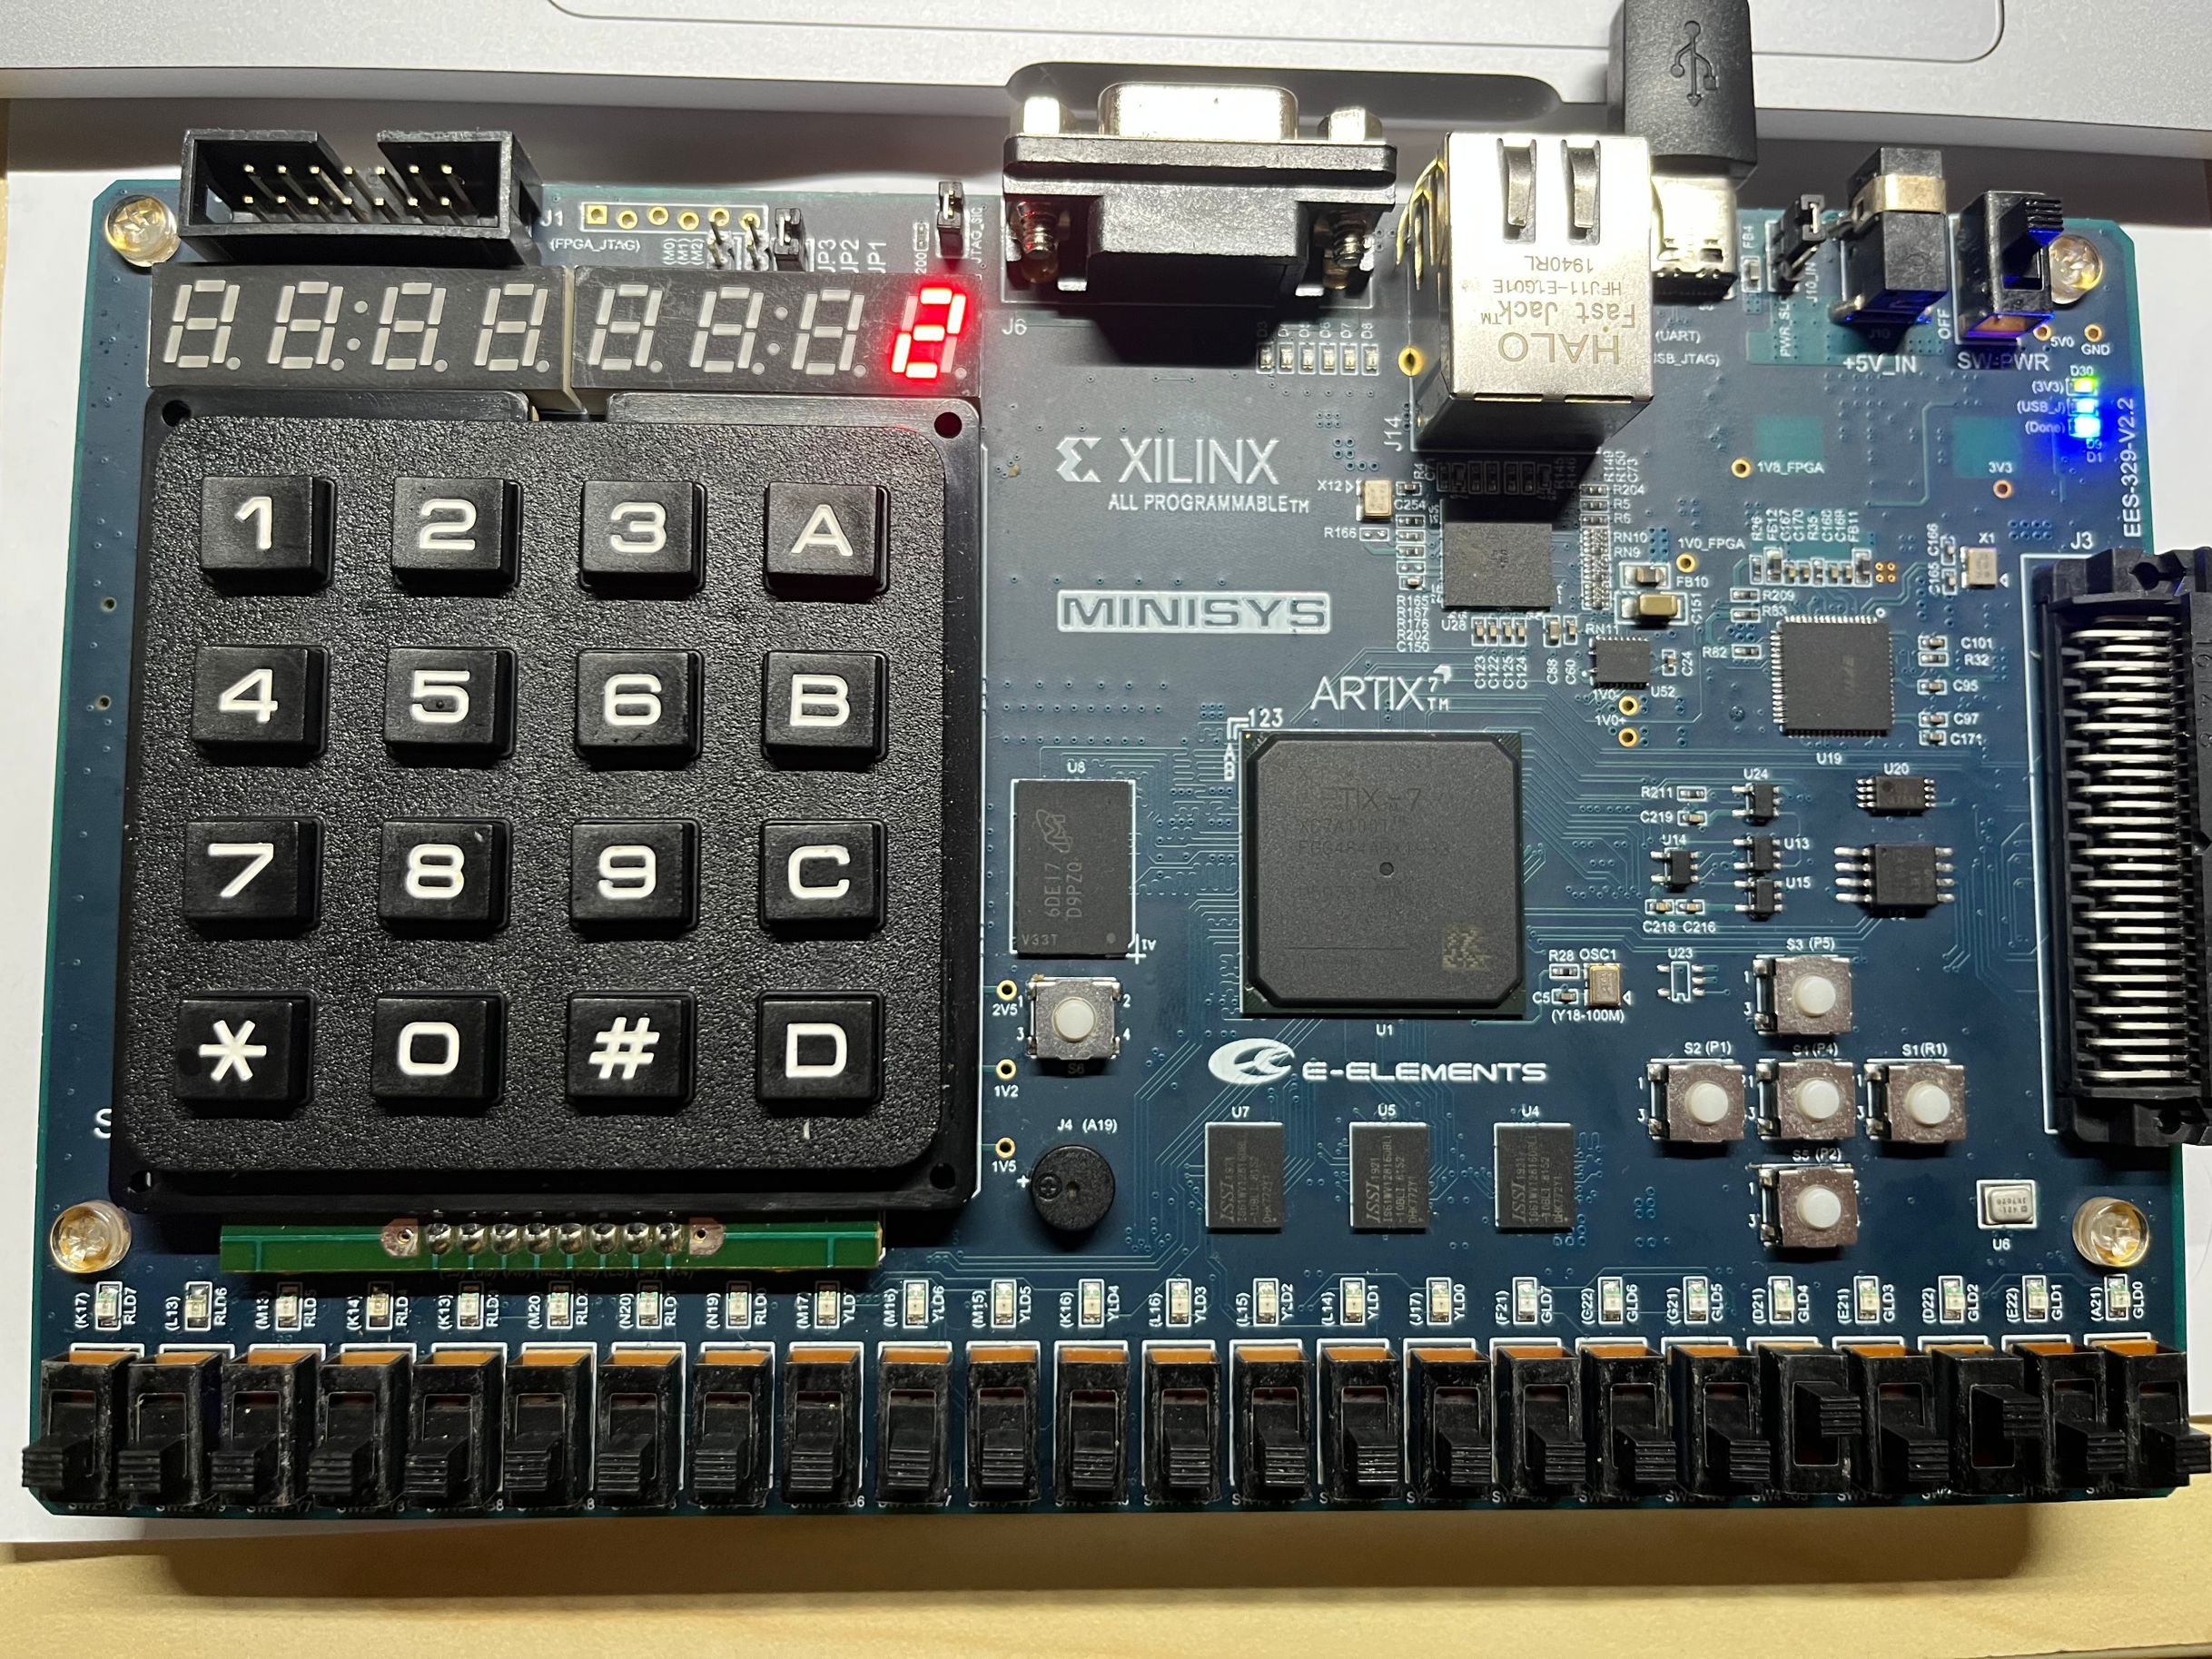
\includegraphics[width=0.35\textwidth]{./t1/hif1.jpg}}
		\caption{Showing in both high/low-first mode, when only one ward calls, display the corresponding room number}
	\end{subfigure}
	\begin{subfigure}[b]{\textwidth}
		\centerline{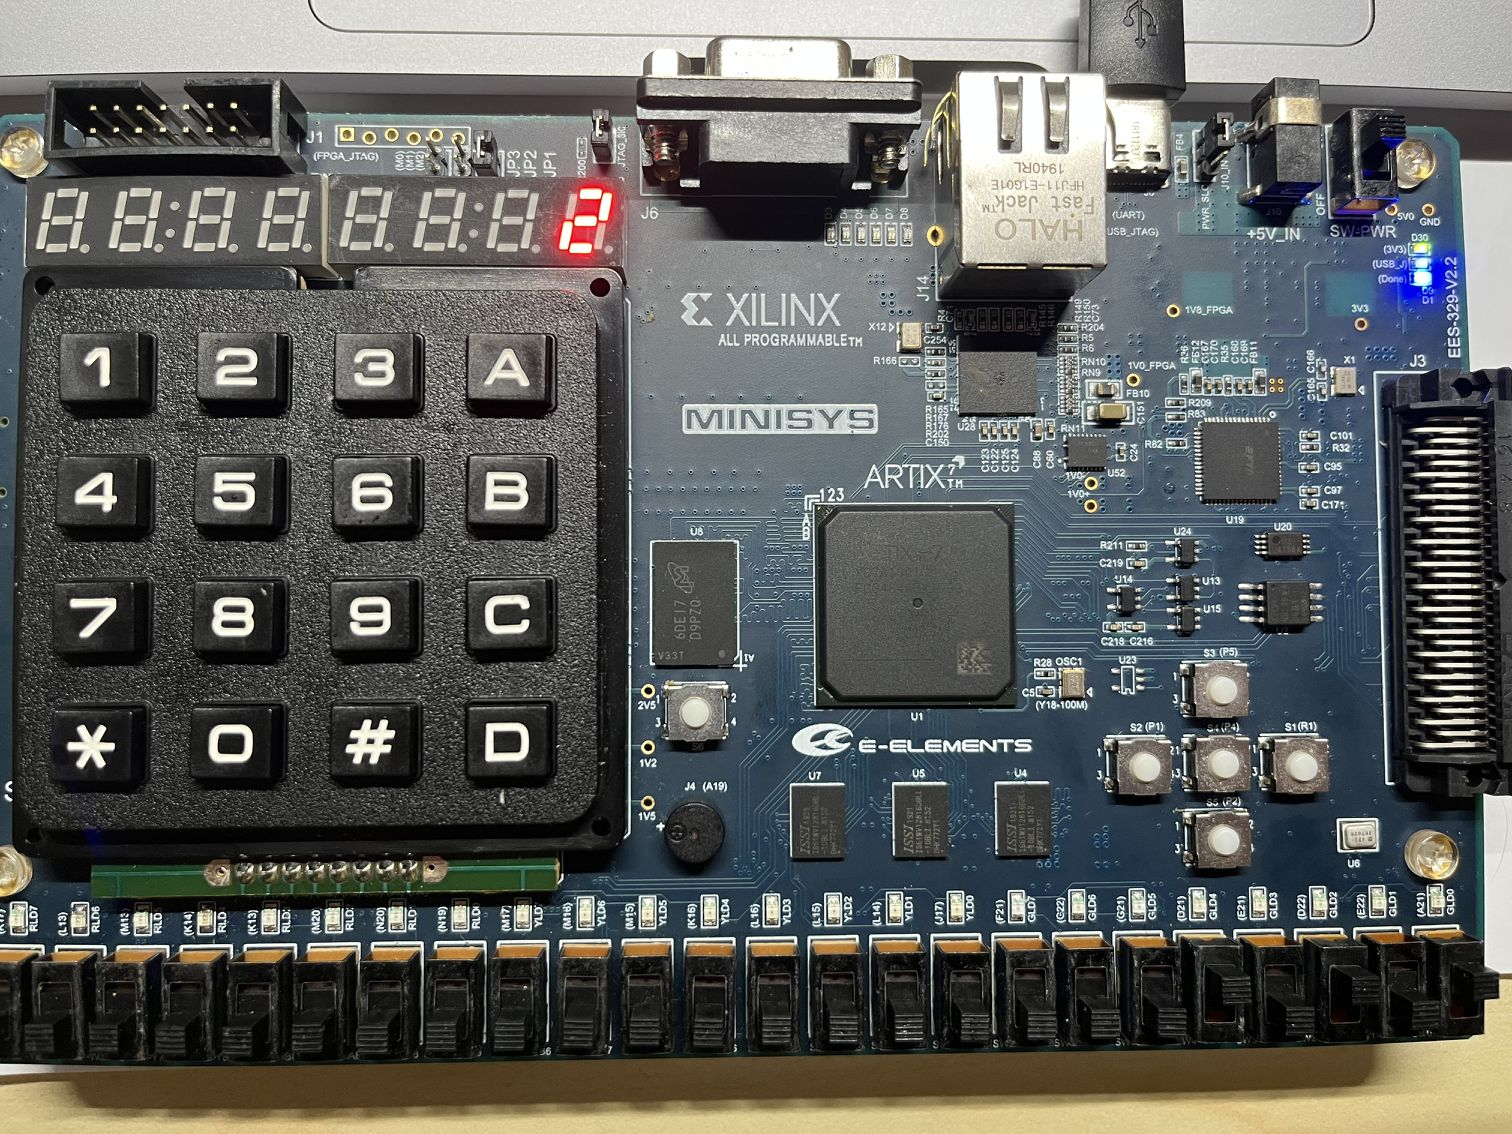
\includegraphics[width=0.35\textwidth]{./t1/hif2.jpg}\qquad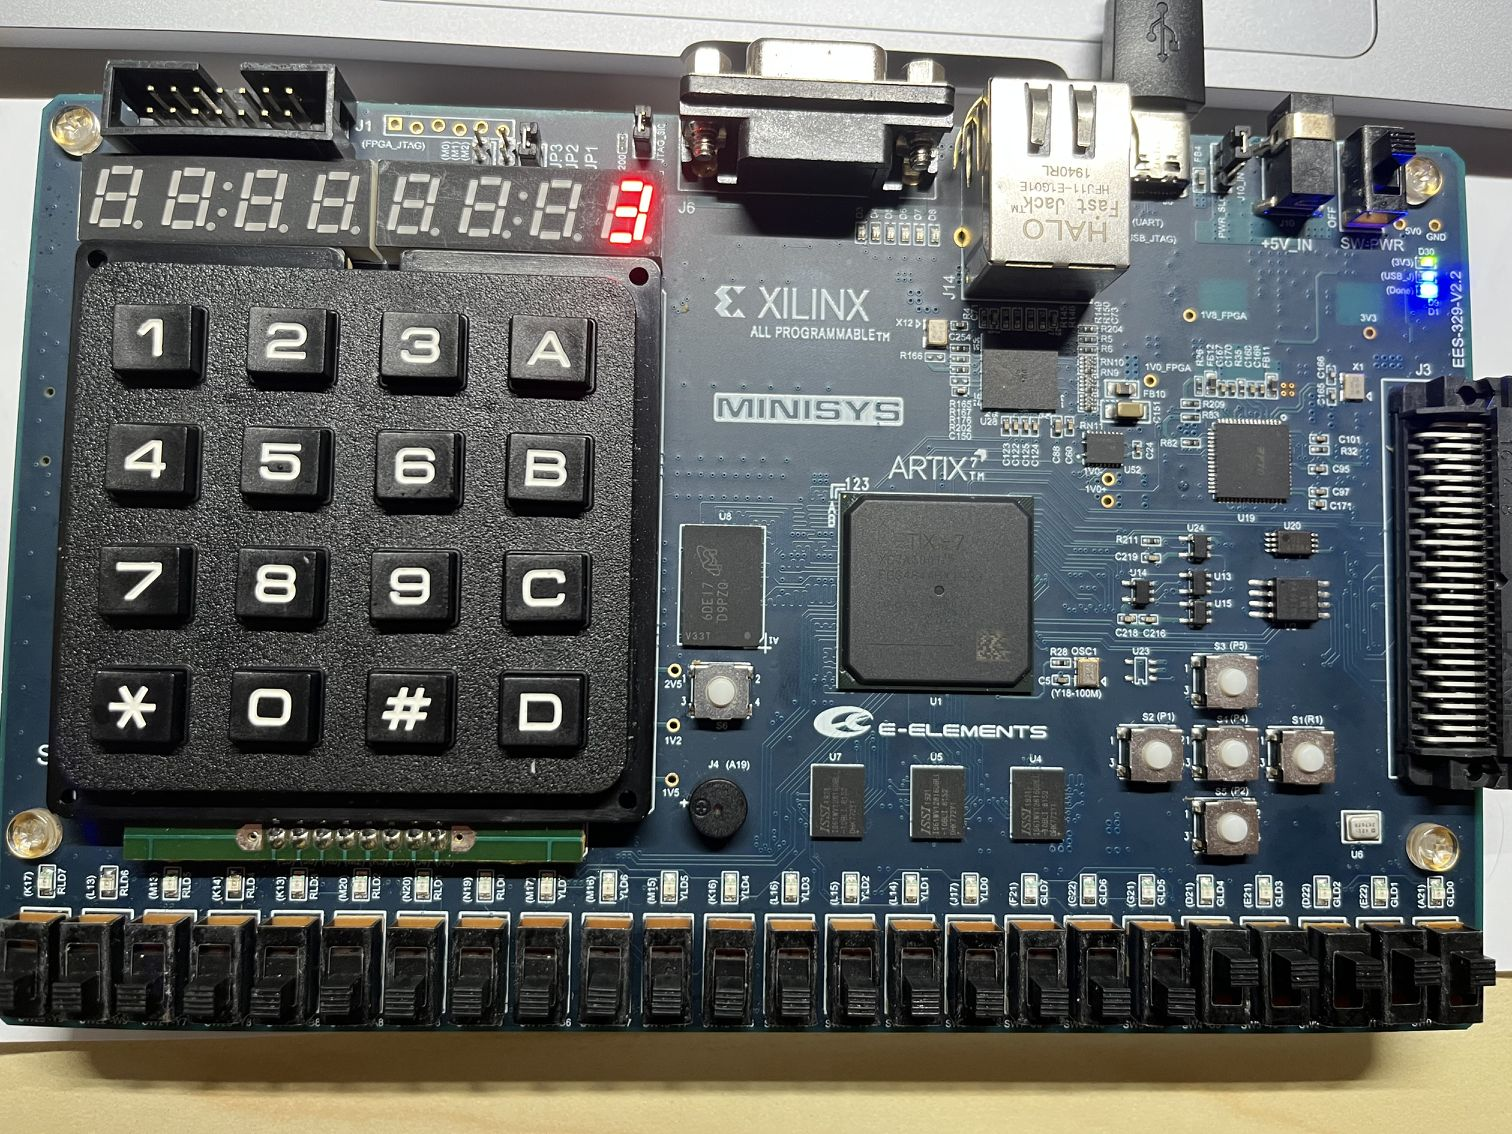
\includegraphics[width=0.35\textwidth]{./t1/hif3.jpg}}
		\caption{Showing in high-first mode, bell 0\&2 on $\to$ display 2; bell 0\&1\&2\&3 on $\to$ display 3}
	\end{subfigure}
	\begin{subfigure}[b]{\textwidth}
		\centerline{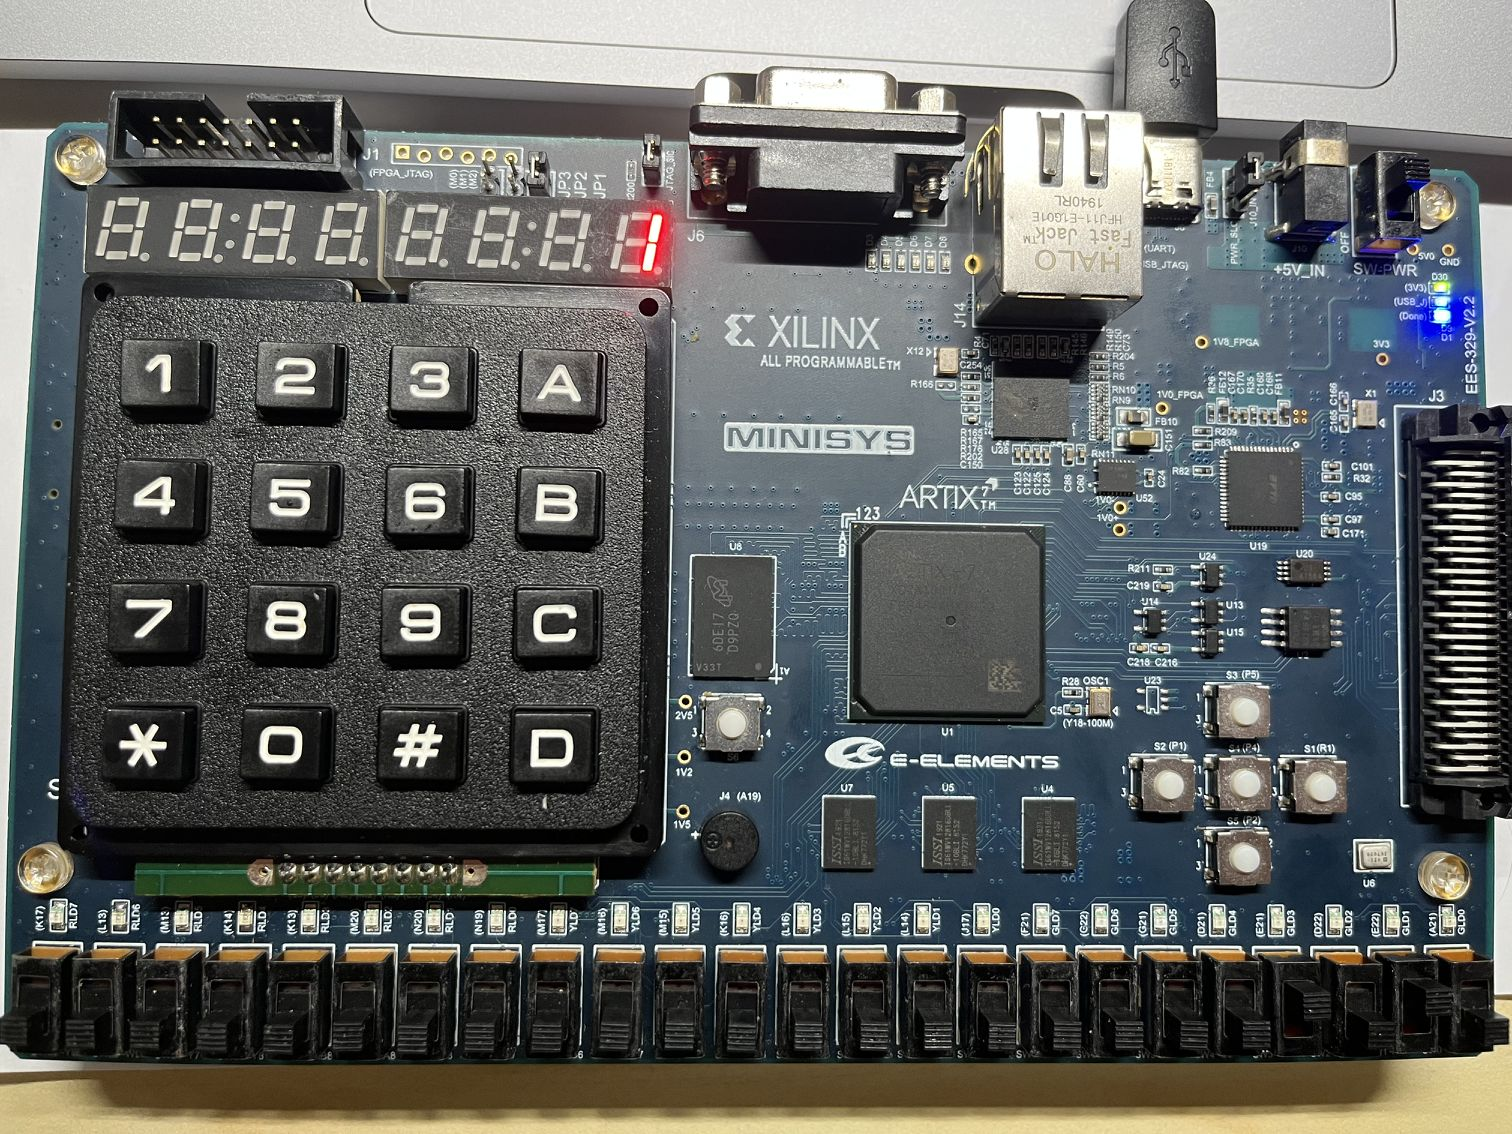
\includegraphics[width=0.35\textwidth]{./t1/lof13.jpg}\qquad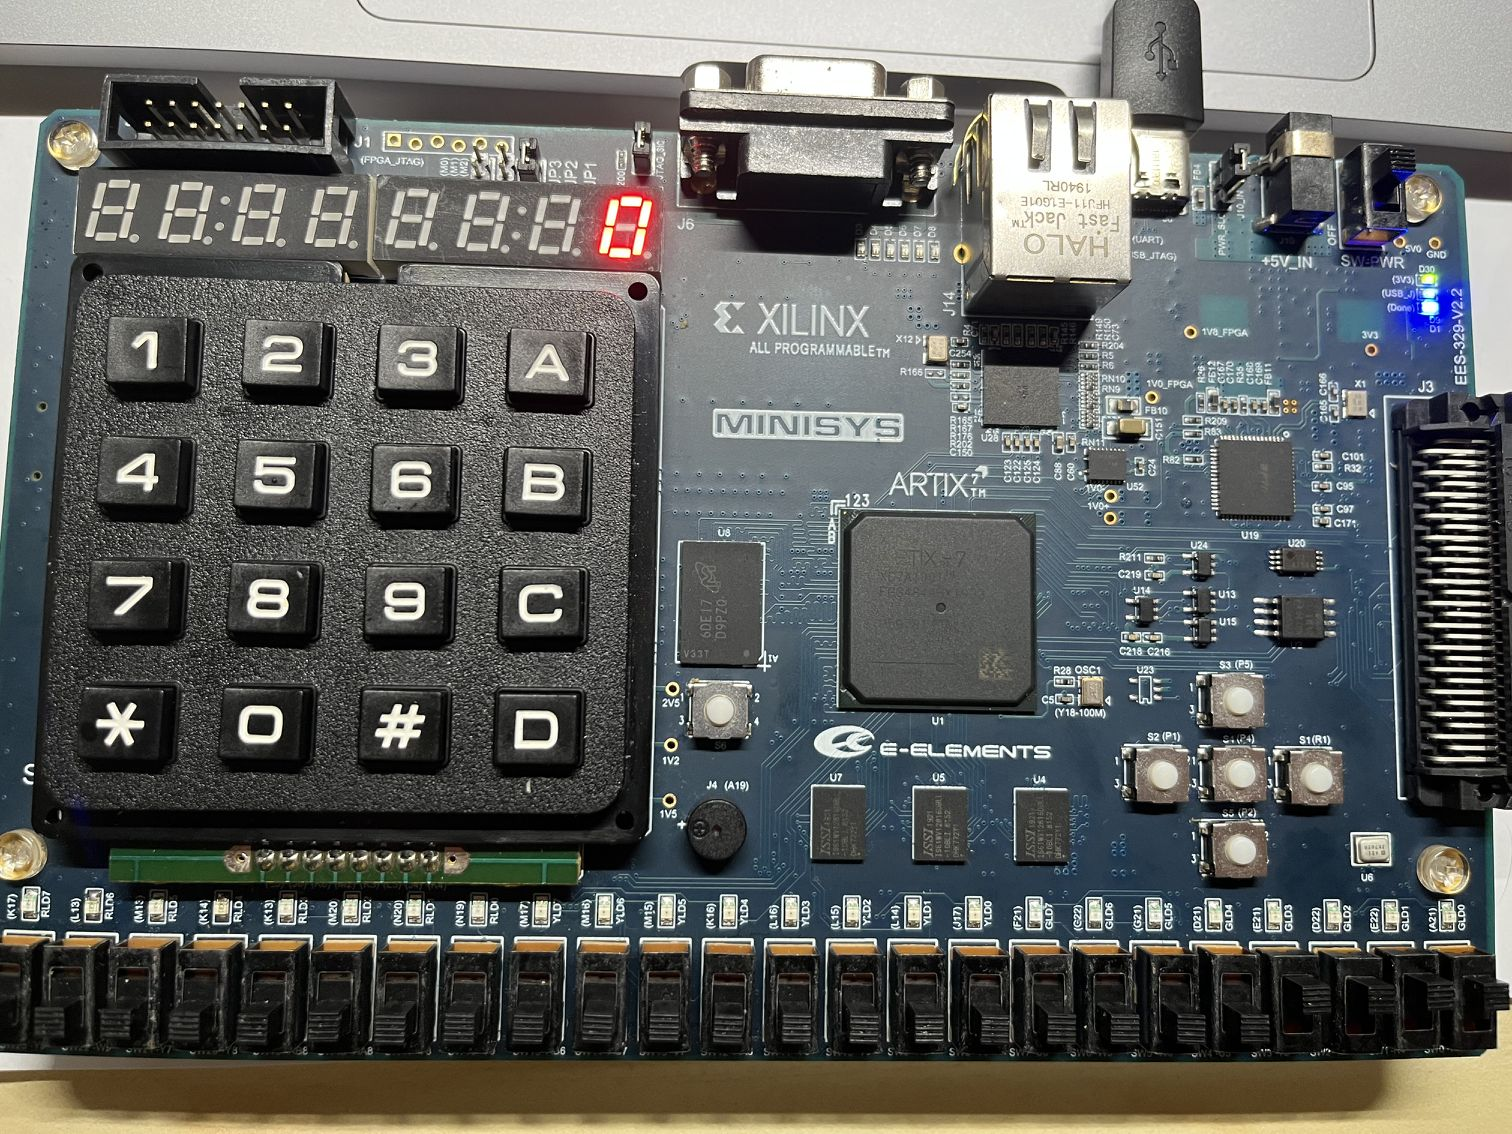
\includegraphics[width=0.35\textwidth]{./t1/lof3.jpg}}
		\caption{Showing in low-first mode, bell 1\&3 on $\to$ display 1; bell 0\&1\&2\&3 on $\to$ display 0}
	\end{subfigure}
	\caption{Verifying Task 1}
	\label{fig:visual_smap}
\end{figure*}
\pagebreak

\subsection{Task 2}
%\scriptsize
%\centerline{Truth Table}
%\normalsize
\begin{table}[H]
\centering
\begin{tabular}{|c|c|c|c|}
\hline
$a$ & $b$ & $c$ & $F(a,b,c)=a\oplus b\oplus c$ \\ \hline
0   & 0   & 0   & 0                            \\ \hline
0   & 0   & 1   & 1                            \\ \hline
0   & 1   & 0   & 1                            \\ \hline
0   & 1   & 1   & 0                            \\ \hline
1   & 0   & 0   & 1                            \\ \hline
1   & 0   & 1   & 0                            \\ \hline
1   & 1   & 0   & 0                            \\ \hline
1   & 1   & 1   & 1                            \\ \hline
\end{tabular}
\end{table}
\begin{center}
\begin{karnaugh-map}[4][2][1][$ab$][$c$]
\minterms{1,2,4,7}
\implicant{1}{1}
\implicant{2}{2}
\implicant{4}{4}
\implicant{7}{7}
\end{karnaugh-map}
\begin{align*}
F(a,b,c)&=a'b'c+a'bc'+abc+ab'c'&\text{(SOP)}\\
&=(a+b+c)(a+b'+c')(a'+b'+c)(a'+b+c')&\text{(POS)}
\end{align*}
\end{center}
\subsubsection*{Design file}
\begin{lstlisting}
`timescale 1ns/1ps

module task2 (
    input a, b, c,
    output sop, pos
);
    assign sop = ~a & ~b & c | ~a & b & ~c | a & b & c | a & ~b & ~c;
    assign pos = (a | b | c) & (a | ~b | ~c) & (~a | ~b | c) & (~a | b | ~c);
endmodule
\end{lstlisting}
\subsubsection*{Simulation file}
\begin{lstlisting}
`timescale 1ns/1ps

module tsk2tb ();
    reg a, b, c;
    wire sop, pos;

    task2 t(a, b, c, sop, pos);

    initial begin
        {a, b, c} = 3'b000;
        while ({a, b, c} < 3'b111)
            #10 {a, b, c} = {a, b, c} + 1;
        #10 $finish();
    end
endmodule
\end{lstlisting}
\vspace{-1.5em}
\centerline{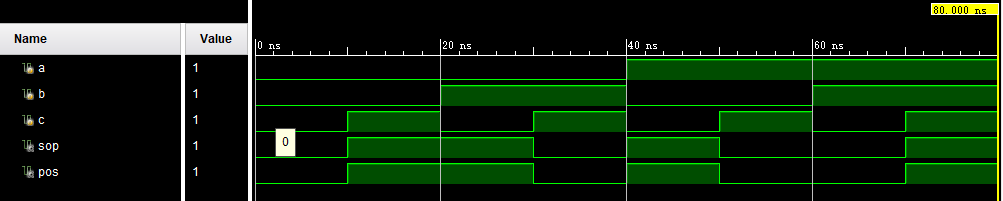
\includegraphics[width=\textwidth]{t2/tsk2}}
\par From the waveform above we see:
\vspace{-1em}
\paragraph{\ding{172}} The truth-values of SOP and POS design are always the same.
\vspace{-1em}
\paragraph{\ding{173}} When the number of \emph{true} in the three variables \textit{a, b, c} is odd, the truth value of $a\oplus b\oplus c$ is \emph{true}, otherwise is \emph{false}. The result keeps the same as the truth table.

\subsection{Problems \& Solutions}
\paragraph{(1)} At first I directly used part of the constraint file (about the seg-tube) provided on the lab scission, then I found there always light up two numbers together. After checking the design file, constraint file and the minisys user manual carefully, I found there's a mis-constrained port and fixed it.
\vspace{-1em}
\paragraph{(2)} Designing the seg-tubes that are low-level effective is no that intuitive and need much care. An intuitive way is designing them in high-level way that use 1 to active one, and add a \emph{bitwise not} to transverse them.
\vspace{-1em}
\paragraph{(3)} Maybe the next assignment could be harder and contains more questions :)

\end{document}